% 一元函数的微分
% 微积分|导数|极限|微分|微分近似

\pentry{导数\upref{Der}}
考察一个连续光滑的函数 $y = f(x)$, 在 $x$ 处函数值为 $y$, 若此时函数增加一个无穷小量 $\dd{x}$, 函数值会相应增加无穷小量 $\dd{y}$. 根据导数的定义\upref{Der} $f'(x) = \dv*{y}{x}$, 我们将 $\dd{y}$ 与 $\dd{x}$ 的关系记为
\begin{equation}\label{Diff_eq1}
\dd{y} = f'(x) \dd{x}
\end{equation}
这就是一元函数的\textbf{微分}.注意一元函数的求导和微分除了表达方式不同外并无太大区别.从形式上来看,微分是微小变化量之间的线性关系,而导数则强调变化率.

\subsection{微分近似}
严格来说,类似\autoref{Diff_eq1} 的微分关系式默认取极限 $\dd{x} \to 0$ 才能使等号成立,但只要在一定范围 $\Delta x$ 内导函数 $f'(x)$ 的变化非常小,就可以将函数值的变化量 $\Delta y = f(x+\Delta x)-f(x)$ 近似为
\begin{equation}\label{Diff_eq2}
\Delta y \approx f'(x) \Delta x
\end{equation}
注意在近似式中不能出现微分符号 $\dd$, 也不能使用等号.

\begin{figure}[ht]
\centering
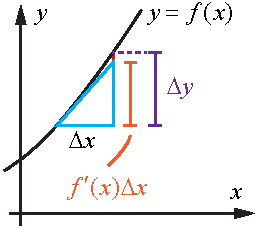
\includegraphics[width=4.5cm]{./figures/Diff1.pdf}
\caption{微分近似用函数曲线的切线增量 $f'(x)\Delta x$ 来近似函数增量 $\Delta y$} \label{Diff_fig1}
\end{figure}

\begin{example}{测量误差}\label{Diff_ex1}
若测得立方体的边长为 $a$, 测量的最大可能误差为 $\sigma_a$ (可以假设 $\sigma_a \ll a$), 估计立方体体积的最大误差 $\sigma_V$.

立方体的体积与边长的关系为 $V(a)=a^3$, 根据微分近似,有
\begin{equation}
\sigma_V \approx V'(a) \sigma_a = 3a^2 \sigma_x
\end{equation}
\end{example}

\begin{example}{细圆环的面积和薄球壳的体积}\label{Diff_ex2}
圆的面积关于其半径的函数为 $A(r) = \pi r^2$, 对该式进行微分得 $\dd{A} = 2\pi r\dd{r}$. 注意到 $2\pi r$ 为 $r$ 对应的周长, 所以该微分式的意义就是, 半径为 $r$, 宽度为 $\dd{r}$ 的圆环的面积等于该圆环的周长乘以圆环的宽度.

球的体积关于其半径的函数为 $V(r) = 4\pi r^3/3$, 求微分得 $\dd{V} = 4\pi r^2 \dd{r}$. 注意到 $4\pi r^2$ 为 $r$ 对应的球表面积, 所以该微分式的意义是, 半径为 $r$, 厚度为 $\dd{r}$ 的球壳的体积等于该球壳的表面积乘以球壳厚度.
\end{example}


